\section{Interpretation and Discussion}
%NEW%%%%%%%%%%%%%%%%%%%%%%%%%%%%%%%%%%%%%%%%%%%%%%%%%%%\text{ [erg s}^{-1}\text{ cm}^{-2}\text{sr}^{-1}\text{ \AA\ }^{-1}]
\subsection{Sunquake Impact Momentum}
The momentum needed to produce the sunquake is,

\begin{equation}\label{sqk-momentum} 
p_{sqk}\sim \rho \; l^{3} \; v \text{ [g cm s}^{-1}]
\end{equation}

\noindent
where all terms are tailored for photospheric values, hence density $\rho \sim 10^{-8}$g cm$^{-3}$; sound speed $v \sim 10^{6}$ cm.s$^{-1}$ \citep{2015ApJ...807..102S}. The length-scale, $l \sim  1.82{\times}10^{8}$ cm, corresponds to the sunquake impact diameter, 

\begin{equation}\label{lengthscale}
l = 2\sqrt{\frac{A_{sqk}}{\pi}} \text{ [cm]}
\end{equation}

%Equation \ref{sqk-momentum} gives the momentum of the acoustic reponse as $p_{sqk} = 6.03{\times}10^{22}$ g cm s$_{-1}$, which when compared to particle beam momenta, $p_e$ and $p_p$, is $10{5}$ and $10^{4}$ times larger respectively. 
\noindent
An alternative method of calculating the momentum associated with the sunquake is to use the $P_{sqk}$. By further developement of equation \ref{sqk-momentum} shown in the Appendices section \ref{sqk-ptoP-relation}, sunquake momentum becomes,  

\begin{equation}\label{sqk-momentum-from-power}
p_{sqk} \; \sim \; \frac{P_{sqk} \; \rho \; v \; l }{F_{sqk}} \text{ [g cm s}^{-1}]
\end{equation}
\noindent
where acoustic emission flux, $F_{sqk} = $ (see equation \ref{Psqk}). A range of velocities can be input into equations,\ref{sqk-momentum} and \ref{sqk-momentum-from-power}, allowing the consideration of lower and upper limits of acoustic impact momentum. The momentum values resulting from inputing sunquake wavefront velocity of $v_{sqk} = 8.0{\times}10^{8}$ cm s$^{-1}$ \citep{2014ApJ...796...85J} and the photospheric sound speed into equations \ref{sqk-momentum} and \ref{sqk-momentum-from-power} are shown in Table \ref{sqk-momenta}. Taking upper and lower limits for calculated acoustic source momentum as $4.73{\times}10^{22} \leq p_{sqk} \geq 4.82{\times}10^{25}$ g cm s$^{-1}$, comparisons can be made with particle beam and radiation pressure momenta.\\
\begin{table}[h]
%\tiny
\centering
\begin{tabular}{|c|c|c|}
Velocity $v$ [cm s$^{-1}$] & Eqn \ref{sqk-momentum} $p_{sqk}$ [g cm s$^{-1}$] & Eqn \ref{sqk-momentum-from-power} $p_{sqk}$ [g cm s$^{-1}$]\\
\hline
$8.0{\times}10^{8}$ (sunquake wave speed) & $4.82{\times}10^{25}$ & $3.79{\times}10^{25}$\\
$1.0{\times}10^{6}$ (photospheric sound speed) & $6.03{\times}10^{22}$ & $4.73{\times}10^{22}$\\
\end{tabular}
\caption{Acoustic impact momenta in cgs units, g cm s$^{-1}$, caclulated using by inputting values shown in the 'Velocity' column into equations \ref{sqk-momentum} and \ref{sqk-momentum-from-power}. These values provide an upper and lower limit on sunquake impact momentum.}\label{sqk-momenta}
\end{table}


\subsection{Partcle Beam}
Using the nonthermal power, $P_{e}$ from the RHESSI data fit detailed in Section \ref{rhessiresults}, the flux input by the nonthermal particle beam can be calculated as,

\begin{equation}\label{electronflux}
F_e = \frac{P_{e}}{A_{HXR}} \text{ [erg s}^{-1}\text{ [cm}^{-2}]
\end{equation}
\noindent
Flux $F_e$ is in units of erg s$^{-1}$ cm$^{-2}$ and the HXR emission area is determined by the $90\%$ HXR contour in Figure \ref{hmicontext}, rendering $A_{HXR} \sim \pi (2"{\times}7.25{\times}10^{7})^{2} = 6.61{\times}10^{16}$ cm$^{2}$. The resulting flux turns out to be $F_e \sim 10^{44}$ erg s$^{-1}$ cm$^{-2}$ which when multiplied by the sunquake area, can provide an upper limit for the nonthermal power available for generating an acoustic disturbance $P_{e}(A_{sqk}) = \frac{F_e}{A_{sqk}}$ erg s$^{-1}$. So using the available nonthermal energy, $P_e \sim 2.5{\times}10^{29}$ erg.s$^{-1}$ and $A_{sqk} \sim 2.6{\times}10^{16}$ $cm^{2}$. $P_{e}(A_{sqk}) \sim 10^{28}$ erg s$^{-1}$ and when compared with the sunquake power $P_{sqk} \sim 1.3\pm0.05{\times}10^{26}$ erg s$^{-1}$ the electron beam has 1000 times more energy than the sunquake. Another interesting quantity to investigate is the momentum of the particle beam. Electron momentum can be calculated by 


\begin{equation}\label{electron-momentum}
p_e=\tau \sqrt{2m_e} P_{e} \text{ [g cm s}^{-1}]
\end{equation}
\noindent
where $m_e$ is electron mass, $\tau$ is the time duration of flare impulsive phase and $P_{e}$ is described by equation \ref{pnth1} \citep{2015ApJ...807..102S}. Substituting values in to equation \ref{electron-momentum} yields an electron momentum of $p_e \sim 1.35{\times}10^{17}$ g cm s$^{-1}$. Assuming the energy in the electron beam is equal to that in a population of accelerated protons \citep{2000ApJ...542..513E}, then calculation of a theoretical proton beam momentum, where $m_p$ is the proton mass, is by the relation,

\begin{equation}\label{proton-momentum}
p_p \sim p_e \sqrt{\frac{m_p}{m_e}} \text{ [g cm s}^{-1}]
\end{equation}
\noindent
Which yields a proton momentum of $p_p \sim 5.79{\times}10^18$ g cm s$^{-1}$, an order of magnitude greater than $p_e$. This is because $m_p ~ 2000m_e$ meaning the square root in equation \ref{proton-momentum} renders the result $p_p \sim 44.7p_e$ g cm s$^{-1}$. Comparing $p_{e}$ and $p_{p}$ with the lower limit of $p_{sqk}$, the electron and proton beam carry $\sim 10^{5}$ and $\sim 10^{4}$ times less momentum than $p_sqk$ respectively. This means that even if an electron or proton beam can make it down to the photosphere, it wouldn't have the necessary momentum to cause the sunquake on its own. In reality, calculated momenta are idealistic, not treating the effects of energy loss due to energy dissapation. The point being that for a particle beam to make it to the photosphere, it has to traverse 9 pressure scale heights, increasing in density with depth. As density increases particles in the beam are more likely to encounter ambient plasma, and as a result are deccelerated, giving up as energy as emission. So if or when the beam reaches the photosphere, much of its energy and momentum has already been dissapated in the chromosphere, making the generation of a sunquake via just the particle beam even more unlikely. \\

\subsection{Radiative Backwarming}
Energy deposited into the atmosphere by the particle beam can lead to other sunquake generation mechanisms, such as radiative backwarming and shocks which are described in sections \ref{sunprog}. A recent result from \cite{2016ApJ...816...88K} shows that the intensity of Balmer continuum observed in this event could come from either; 23\% of nonthermal electrons with energy $<20$ keV; or the entire population of nomthermal electrons with energy $<40$ keV. This means that a large portion of energy delivered to the lower atmosphere by the electron beam is dissapated causing various continua and emission lines. \\
\noindent
The flux values for Balmer and HMI continuum shown in Figure \ref{fluxladder-balm-hmi-only} can be used to estimate the power of the radiative backwarming. The key being whether the radiative backwarming is powerful enough to generate the white light flare and hence the sunquake. The power profiles shown in Figure \ref{powerladder-balm-hmi-only} are calculated by assuming a homogenous energy distribution in the region surrounding each coordinate, it is then possible to use the relation,

\begin{equation}
P_{Balm} = F_{Balm} \; A_{sqk}  \text{ [erg s}^{-1}]
\end{equation}\label{Pbalm}
\noindent
where $P_{Balm}$ is the power of the Balmer continuum emitted from an area equal to the sunquake, $A_{sqk}$. The same data set and coordinate scheme is followed as in Figure \ref{fluxladder-balm-hmi-only}. The Balmer continuum over the sunquake shows an impulsive power $P_{Balm} = 6{\times}10^{13}$ erg s$^{-1}$ which is thirteen orders of magnitude smaller than the power of the sunquake $P_{sqk} \sim 1.3\pm0.05{\times}10^{26}$ erg s$^{-1}$. This means that there is not enough energy per second deposited by radiative backwarming to create the sunquake. The HMI continuum power, $P_{HMI}$, over the sunquake location peaks at $P_{HMI} = 2{\times}10^{14}$ erg s$^{-1}$cm$^{-2}$, which is twelve orders of magnitude less than the $P_{sqk}$ but ten times greater than the Balmer continuum. One of the biproducts of radiative backwarming are white light flares in the photosphere. Balmer continuum radiated outward to the observer, is supposed to be equal in power to that emitted downward \citep{1989SoPh..124..303M}. In that case the white light flare shown in the HMI continuum in Figure \ref{powerladder-balm-hmi-only} is only provided $10\%$ of its power by radiatve backwarming. So radiative backwarming at first glance may not be causing the observed white light emission.

\begin{figure}[H]
  \begin{center}
  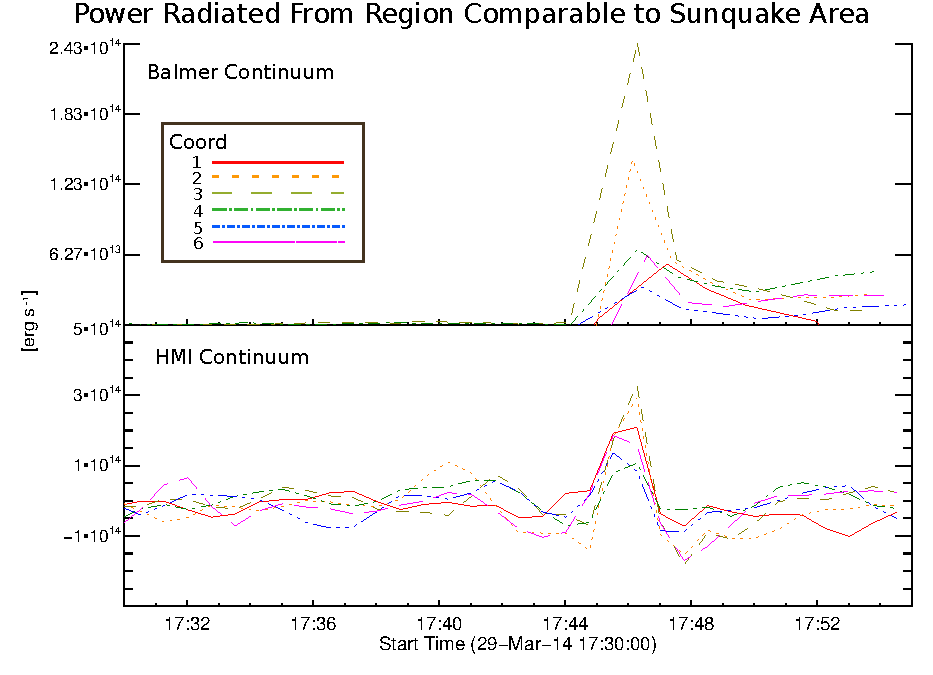
\includegraphics[width=0.9\textwidth]{29-Mar-14-A_sqk-Power-Ladder-Balm-HMI-Only}
  \end{center}
  \caption{Shows radiative power [erg s$^{-1}$], which is the result of flux data that has been multiplied by the sunquake impact area. The six lines (see legend) represent areas centered on regions 1 to 6, relating to heliocentric coordinates shown in Table \ref{coordtab}. The solid red line is directly over the sunquake location. The top plot is IRIS SG  2825.7 to 2825.8 Balmer Continuum and the bottom plot is SDO HMI continuum.}\label{powerladder-balm-hmi-only}
\end{figure}

\noindent
However, another way to investigate the energy deposition in the lower atmosphere is by integrating radiative flux over the impulsive phase of the flare. This provides an upper limit for the total flux injected into the system during the impulsive phase, which can be used to calculate the total emission power. The integrated flux is calculated,

\begin{equation}
F_{imp} = \int_{0}^{\tau} F(t) \; dt = F(t) \; \tau \text{ [erg cm}^{-2}]
\end{equation}\label{f-imp}
\noindent
where the duration of the impulsive phase $\tau = $ and $F(t)$ is the emitted flux at time $t$. The total energy emitted during the impulsive phase, $E_{imp}$ is

\begin{equation}
E_{imp}=F_{imp} \; A_{sqk} \text{ [erg}]
\end{equation}\label{e-imp}
\noindent
where it is assumed that a homogenous energy distribution exists throughout the sunquake impact area. This produces values for each data set tabulated in Table \ref{eimp}. 


\begin{table}[h]
%\tiny
\centering
\begin{tabular}{|c|c|c|c|c|c|c|c|c|c|c|}
Coord Number & Coorinates (x,y) [arcsecs] & $E_{Si IV}$ [erg] & $E_{Mg II}$ [erg] & $E_{Balm}$ [erg] & $E_{Mg II w}$ [erg] & $E_{HMI}$ [erg]\\
\hline
1 & 518.22, 262.00 & 6.74E+12 & 1.41E+14 & 5.98E+15 & 4.27E+12 & 1.42E+16\\
2 & 520.22, 263.00 & 5.65E+12 & 1.35E+14 & 1.71E+16 & 7.14E+12 & 1.10E+15\\
3 & 522.21, 262.00 & 5.18E+12 & 7.83E+13 & 2.52E+16 & 2.91E+12 & 4.82E+15\\
4 & 522.21, 265.00 & 3.93E+12 & 8.35E+13 & 9.89E+15 & 6.70E+13 & 1.28E+15\\
5 & 524.26, 265.00 & 3.98E+12 & 1.03E+14 & 4.37E+15 & 1.86E+13 & 8.99E+14\\
6 & 526.25, 263.82 & 6.91E+12 & 6.34E+13 & 5.24E+15 & 1.74E+12 & 9.88E+14\\
\end{tabular}
\caption{Flux integrated over the flare impulsive phase (17:44 to 17:48) is then multiplied by the sunquake impact area to produce a total deposited energy in erg. The values show are for ribbon sample locations 1 to 6.}\label{eimp}
\end{table}
\noindent
Balmer and HMI continua are the data sets that show the highest integrated energy levels, with comparable values at each coordinate. The fact that Balmer and HMI continua show such similar energies emitted over the impulsive phase means that radiative backwarming is likely causing the white light flare in the photosphere as described in section \ref{wlf}. The highest energy reading in the HMI continuum is over the sunquake, with a value of $1.42{\times}10^{16}$ erg whereas in the Balmer continuum the highest is coordinate three with $2.52{\times}10^{16}$ erg, both of which are ten orders of magnitude smaller than $P_{sqk}$. For the sake of rigor in interpreting the radiative backwarming contribution, it can also be measured in terms of radiation momentum, $p_{rad}=\frac{E}{c}$ g cm s$^{-1}$, where $E$ is the emitted energy in erg and $c$ is the speed of light in cm s$^{-1}$. Using the integrated Balmer continuum energy value from Table \ref{eimp}, the radiation pressure is $p_{rad} = 2.0{\times}10^{5}$ g cm s$^{-1}$, which is $10^{17}$ times smaller than $p_{sqk}$. Meaning that the radiative backwarming mechanism in this case is not powerful enough to produce the sunquake. \\ 

\section{Conclusions and Thesis Plan}
Calculations estimate that the sunquake is generated by an input momentum in the range $4.73{\times}10^{22} \leq p_{sqk} \geq 4.82{\times}10^{25}$ g cm s$^{-1}$. 50 to 100 keV HXR measurements show the impulsive phase of the flare occurs from 17:46 to 17:47. HXR contours and nonthermal power curve show that there is a energetic particle beam directly over the sunquake. When compared to the sunquake power the nonthermal electron beam has 1000 times more energy, which is enough to cause the sunquake. However, further inspection reveals that the electron beam has insufficient by five orders of magnitude in momentum to generate the sunquake. A proton beam is also considered, this is a theoretical upper limit calculation of the momentum carried by such a beam. It turns out that the proton beam is also lacking the momentum to cause the sunquake by four orders of magnitude. For these reasons it is unlikely that a nonthermal particle beam is capable of producing a sunquake in this event. Instead, nonthermal energy is deposited in the lower solar atmosphere giving rise to various emission. The Balmer continuum sampled from the sunquake location emits at a power that is thirteen orders of magnitude smaller than the power of the sunquake. Whilst radiative backwarming radiation momentum calculations yield a result that is seventeen orders of magnitude to small. These calculations performed on the Balmer continuum data show that there is not enough energy or momentum in the radiative backwarming to generate the sunquake. HMI continuum sampled from the sunquake location emits at a power which is lacking by twelve orders of magnitude when compared to that needed to produce the sunquake. Also HMI continuum emits approximately ten times more power than Balmer continuum, meaning it is unlikely that radiative backwarming is causing the white light flare. Energies integrated over the impulsive phase of the flare for Balmer and HMI continua show a similar results. Both being short of energy by ten orders of magnitude, reiterating that radiative backwarming is not generating the sunquake. There must be some other energy source involved in producing the acoustic source. \\
\noindent
From the analysis, it is clear that the sunquake is unlikely to be caused by either a particle baem or radiative backwarming, so what else could be causing the sunquake? \cite{2015ApJ...812...35M} show that during the impulsive phase there is substantial redshifted in many IRIS SG spectral lines over the sunquake location, indicating the existence of a shock. Momentum associated with a downward shock is predicted to be instigated by a nonthermal electron beam or the presence of Alfven waves. Another possibility is sunquake production via a transient Lorentz force caused by the reconfiguring magnetic field. However, \cite{2014ApJ...796...85J} show that the change in magnetic field over the sunquake is not large enough to generate a sufficient Lorentz force capable of producing the sunquake. A purely theoretical idea could be in the form of MHD waves. Dissapation of Alfven waves \citep{1982SoPh...80...99E} has potential as a possible energy transport mechanism maybe capable of producing a sunquake \citep{2015ApJ...812...35M}. Energy in the form of Alfven waves could potentially propagate downward through the solar atmosphere, along the magnetic field. These waves are said to experience with little in the way of dissapation until reaching the temperature minimum region in the upper-photosphere. At which point Alfven waves are dissapated, heating photospheric plasma and causing white light flares. Observation of these waves is challenging, however there have been reports of associated signatures seen in the corona \citep{2009A&A...501L..15B}. 

%radiative backwarming conclusions
\subsection{Thesis Plan}
\noindent
\textbf{Project:} Lower Atmospheric Signatures in a Solar Flare Associated with Seismicity\\
Duration: September 2014 until April/May 2016\\
\noindent
\textbf{Project 2:} Sunquakes; A Statistical Study\\
Starting in April/May 2016 and lasting until February 2017, the idea for this project is a statistical overview of many sunquake events, by developing new tools and using those developed in the first project. Using SDO AIA and HMI, physical properties such as energy, momentum, plasma velocity and magnetic lorentz force will be determined for each event, providing an extensive investigation into the nature of sunquakes. Using a combination of available spacecraft data from RHESSI, Hinode, SDO and IRIS allows the solar atmosphere to be sampled at various emission wavelengths, which can provide information regarding energy and momentum deposition through the solar atmosphere. This information will be used to characterize and catalogue each sunquake observation. A project of this kind will help to increase our knowledge of solar flare energy deposited and generation mechanisms for sunquakes.\\
\noindent
\textbf{Project 3:} Is Energy Dissipation of Alfven Waves in the Lower Solar Atmosphere Capable of Producing a Sunquake? \\
Starting sometime between April/May 2016 and February 2017, this project will probably run parallel with Project 2. The main aim is to search for observational signatures of Alfven waves during solar flares that generate sunquakes. The literature describes dissapation of Alfven waves as producing white light flares \citep{1982SoPh...80...99E, 2013AGUFMSH51A2091F}. Using SDO HMI the energy output of white light flares can be measured. Spectrometers such as EIS and IRIS SG can be used to search for Alfven wave signatures. Comparing HMI continuum energy measurements to energy carried by Alfven waves derived from spectroscopic datas will provide much needed insight into these illusive MHD waves. Results from such a study stands to advance our understanding of the role Alfven waves play in generating white light flares and sunquakes.   




